% resumen_k_tsp_15.0.tex  —  versión final (OPSEARCH / Springer Nature)
%%%%%%%%%%%%%%%%%%%%%%%%%%%%%%%%%%%%%%%%%%%%%%%%%%%%%%%%%%%%%%%%%%%%%%%%%%%
%  Springer Nature LaTeX template (sn-jnl) -- OPSEARCH submission
%  Reference style: sn-chicago (author-year, natbib: \citet / \citep)
%
%  HOW TO COMPILE (Overleaf):
%    1. New Project -> Templates -> "Springer Nature LaTeX Template"
%       (this provides sn-jnl.cls and the sn-*.bst files).
%    2. Upload THIS file (sn-article.tex), body.tex, sn-bibliography.bib,
%       tab_comparacion_global.tex, tab_wilcoxon.tex and the figs/ folder.
%    3. Set sn-article.tex as the main document and Recompile.
%  Compiler: pdfLaTeX. If you prefer strict APA, change sn-chicago to sn-apa
%  (narrative citations may then need apacite's \citeA instead of \citet).
%%%%%%%%%%%%%%%%%%%%%%%%%%%%%%%%%%%%%%%%%%%%%%%%%%%%%%%%%%%%%%%%%%%%%%%%%%%
\documentclass[sn-chicago]{sn-jnl}

\usepackage{graphicx}
\usepackage{amsmath,amssymb,amsfonts}
\usepackage{booktabs}
\usepackage[ruled,vlined]{algorithm2e}
\usepackage{textcomp}
\usepackage{url}

\raggedbottom

\begin{document}

\title[Heuristic approaches for the $k$-TSP]{Heuristic Approaches for the
$k$-Traveling Salesman Problem: A Reproducible Comparison on the TSPLIB Benchmark}

\author[1]{\fnm{Nicol\'as} \sur{Barrientos}}\email{nbarrientos8000@gmail.com}

\author*[1]{\fnm{Gustavo} \sur{Gatica}}\email{ggatica@unab.cl}

\affil[1]{\orgdiv{Facultad de Ingenier\'ia}, \orgname{Universidad Andr\'es Bello},
\orgaddress{\city{Santiago}, \country{Chile}}}

\abstract{The $k$-Traveling Salesman Problem ($k$-TSP) generalizes the classical
Traveling Salesman Problem: given $n$ cities with a home city and a fixed value
$k$ ($1<k\le n$), one must select exactly $k$ cities and order them into a single
closed tour of minimum length, so that the problem couples a selection decision
with an ordering decision. We present a reproducible comparison of ten solution
methods for the $k$-TSP, built on a common local-search core: a greedy
cheapest-insertion heuristic, GRASP, a genetic algorithm, the Nearest Neighbor and
Nearest, Farthest and Random Insertion heuristics, Simulated Annealing, Tabu Search,
and a proposed Deterministic Cheapest-Insertion Heuristic (DCIH). The methods are
evaluated on the 76 TSPLIB instances and the short-/long-run time protocol of
Pandiri and Singh (2020), using the Lin--Kernighan--Helsgaun solver (LKH-3) as the
best-known-solution reference and the two-tailed Wilcoxon signed-rank test for the
statistical analysis. Averaged over all scenarios, the greedy heuristic and Tabu
Search are the most robust of our methods and are significantly better than the
GVNS of that study under both time budgets; under the short run the greedy heuristic
also matches or exceeds the HH\_GREEDY hyper-heuristic, while the randomized
hyper-heuristic remains the strongest overall. The results show that simple,
reproducible heuristics are competitive with dedicated metaheuristics on this
benchmark.}

\keywords{$k$-traveling salesman problem, heuristics, metaheuristics, tabu search,
TSPLIB benchmark, Wilcoxon signed-rank test}

\maketitle

% ============================================================
%  BODY of the k-TSP paper (shared by the Springer wrapper and
%  the local validation wrapper). Citations use natbib (\citep/\citet).
% ============================================================

\section{Introduction}\label{sec:intro}

The $k$-Traveling Salesman Problem ($k$-TSP) is a generalization of the classical
Traveling Salesman Problem (TSP) that has received growing attention in the
combinatorial optimization literature \citep{venkatesh2018,pandiri2020,ene2017,blanchard2023}.
Unlike the standard TSP, in which a single salesman must visit \emph{all} the
cities, in the $k$-TSP the salesman visits only a \emph{subset} of exactly $k$
cities (including a fixed home city) and the remaining $n-k$ cities are left
unvisited. The objective is to minimize the total length of the single resulting
closed tour.

Formally, given $n$ cities with a designated home city (depot) and a fixed value
$k$ with $1 < k \le n$, a feasible solution is obtained by first \emph{selecting}
which $k$ cities to include (the home city among them) and then determining a
\emph{circular ordering} of those $k$ cities \citep{venkatesh2018}. This dual
(selection $+$ ordering) nature distinguishes the $k$-TSP from the standard TSP
and is the source of its combinatorial difficulty: choosing a subset of $k$ nodes
among $n$ and then ordering them yields a search space that grows combinatorially,
making exhaustive enumeration intractable for medium and large instances
\citep{lawler1985}. The TSP is recovered as the special case $k=n$, so the $k$-TSP
is NP-hard \citep{rego2011tsp}.

The $k$-TSP also sits within the broader family of \emph{TSP with profits} and
selective routing problems \citep{feillet2005profits}. In particular, it is the
unit-prize special case of the Quota TSP, itself a variant of the Prize-Collecting
TSP introduced by \citet{balas1989pctsp}: when every node carries a unit prize and
the quota equals $k$, collecting the quota is exactly visiting $k$ nodes
\citep{bienstock1993pctsp}. A recent systematic survey of TSP variants places these
selective problems in a common definitional framework \citep{tspt3co2025}.

Beyond the selective-routing framing, a large body of work targets the classical
TSP itself. Exact methods based on integer and dynamic programming solve it
optimally but scale poorly with $n$ \citep{dantzig1954,bellman1962,heldkarp1962,karp1972},
which motivated decades of research on construction heuristics and local search
\citep{lin1965,christofides1976,bentley1992,johnson1997,laporte1992}. Representative
metaheuristic families include tabu search \citep{glover1986,gloverlaguna1997,knox1994},
simulated annealing \citep{cerny1985}, ant colony optimization \citep{dorigo1997acs},
variable neighborhood search \citep{mladenovic1997vns} and iterated local search
\citep{martin1991}, as well as evolutionary approaches for the TSP
\citep{potvin1996}; broad overviews and design principles are given in
\citep{blumroli2003,talbi2009}. Comprehensive treatments of the TSP and its
variants \citep{gutin2007book}, near-optimal exact solvers
\citep{applegate2006concorde} and polynomial-time approximation schemes for the
Euclidean case \citep{arora1998} complete this landscape, within which
node-selection variants such as the multiple TSP \citep{bektas2006} and the $k$-TSP
naturally arise.

For the $k$-TSP specifically, \citet{venkatesh2018} proposed a general variable
neighborhood search (GVNS) heuristic, and \citet{pandiri2020}, in this journal,
introduced the first metaheuristic and hyper-heuristic approaches (GVNS and two
hyper-heuristics, HH\_RAND and HH\_GREEDY) together with a benchmark of 76 TSPLIB
instances that has since become the reference testbed. The present study adopts
exactly that benchmark and experimental protocol, so that our results are directly
comparable with those of \citet{pandiri2020}.

The main motivation for studying the $k$-TSP lies in applications where only a
subset of locations must be served under a budget on the number of stops:
selective sampling, prize-collecting routing, surveillance with limited visits,
and resource-constrained logistics \citep{vansteenwegen2011top,blanchard2023}.

\paragraph{Contribution.} This work contributes (i) a reproducible, open
implementation that models and solves the $k$-TSP with \emph{ten} methods under a
common local-search core, namely a greedy cheapest-insertion heuristic, a
GRASP/multi-start scheme, a genetic algorithm (GA), the classical Nearest Neighbor
(NN) and Nearest, Farthest and Random Insertion heuristics (NI, FI, RI), Simulated
Annealing (SA), Tabu Search (TS), and a proposed Deterministic Cheapest-Insertion
Heuristic (DCIH); (ii) an evaluation on the 76-instance benchmark of
\citet{pandiri2020} under their short- and long-run time protocol, using the
Lin--Kernighan--Helsgaun solver (LKH-3) as the best-known-solution reference; and
(iii) a statistical comparison, via the two-tailed Wilcoxon signed-rank test,
against the published GVNS and hyper-heuristic results. The remainder of the paper
presents the problem and model (Section~\ref{sec:model}), the solution methods
(Section~\ref{sec:methods}), the experimental setup (Section~\ref{sec:setup}), the
results and discussion (Section~\ref{sec:results}) and the conclusions
(Section~\ref{sec:conclusions}).

\section{Problem definition and mathematical model}\label{sec:model}

The $k$-TSP must choose \emph{which} $k$ nodes to visit and \emph{in which order}.
The number of candidate subsets is $\binom{n-1}{k-1}$ and each admits $(k-1)!/2$
distinct tours; for $n=100$ and $k=50$ the number of subsets alone exceeds
$10^{28}$, so heuristic and metaheuristic methods are required.

Let $G=(V,E)$ with $V=\{0,1,\dots,n-1\}$ and node $0$ the home city (depot), and
let $c_{ij}$ be the distance between nodes $i$ and $j$. We use a single-salesman
selective formulation with two families of binary variables: $y_i=1$ if node $i$
is \emph{selected} (visited) and $0$ otherwise; and $x_{ij}=1$ if the tour
traverses arc $(i,j)$ and $0$ otherwise. Ordering variables $u_i$
(Miller--Tucker--Zemlin, \citealp{miller1960mtz}) eliminate subtours among the
selected nodes. The model minimizes the total tour length
\begin{equation}
\min\ Z = \sum_{i\in V}\sum_{\substack{j\in V\\ j\neq i}} c_{ij}\,x_{ij},
\end{equation}
subject to the selection cardinality (exactly $k$ nodes, home city included)
\begin{align}
\sum_{i\in V} y_i = k, \qquad y_0 = 1,
\end{align}
the degree constraints linking arcs to selection
\begin{align}
\sum_{\substack{j\in V\\ j\neq i}} x_{ij} = y_i, \qquad
\sum_{\substack{j\in V\\ j\neq i}} x_{ji} = y_i, \qquad \forall\, i\in V,
\end{align}
and the MTZ subtour-elimination constraints over the selected nodes
\begin{align}
u_0 = 0,\quad 1 \le u_i \le k-1\ \ \forall i\neq 0,\quad
u_i - u_j + (k-1)\,x_{ij} \le k-2\ \ \forall\, i,j\neq 0,\ i\neq j,
\end{align}
with $x_{ij},y_i\in\{0,1\}$ and $u_i\ge 0$. This is a selective single-tour TSP: it
differs from the standard TSP by the selection variables $y_i$ and the cardinality
constraint $\sum_i y_i=k$, and from the multiple-TSP by having a single salesman.
Related selective routing models (orienteering, prize-collecting) share the
node-selection mechanism \citep{vansteenwegen2011top,gunawan2016op}; the $k$-TSP
fixes the number of visits to exactly $k$ and minimizes length, as defined by
\citet{venkatesh2018}.

\begin{figure}[t]
    \centering
    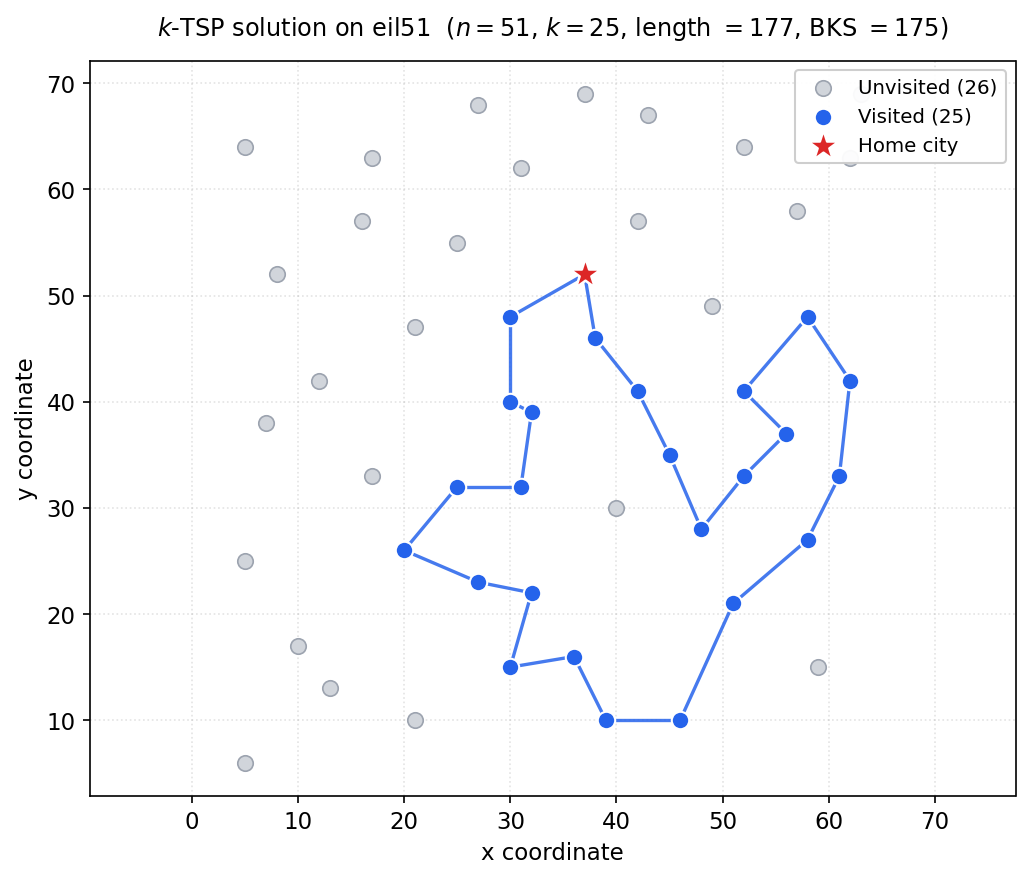
\includegraphics[width=0.6\linewidth]{figs/Graficok-TSP.png}
    \caption{A $k$-TSP solution on \texttt{eil51} with $k=25$ ($\lfloor n/2\rfloor$).
    A single tour (blue) through the home city (red star) visits the $k$ selected
    nodes; the remaining $n-k$ nodes (gray) are left unvisited}
    \label{fig:eil51}
\end{figure}

\section{Solution methods}\label{sec:methods}

All methods share a common representation and local-search core, which makes the
comparison fair. A solution is encoded by the selected subset of $k$ nodes and
their cyclic order (a genotype that decodes into a single closed tour through the
home city, Fig.~\ref{fig:genphen}). The common refinement combines a 2-opt move
over the cycle \citep{croes1958} with an \emph{in/out exchange} that replaces a
selected node by an unselected one, so that both the ordering and the selection
are improved.

\begin{figure}[t]
    \centering
    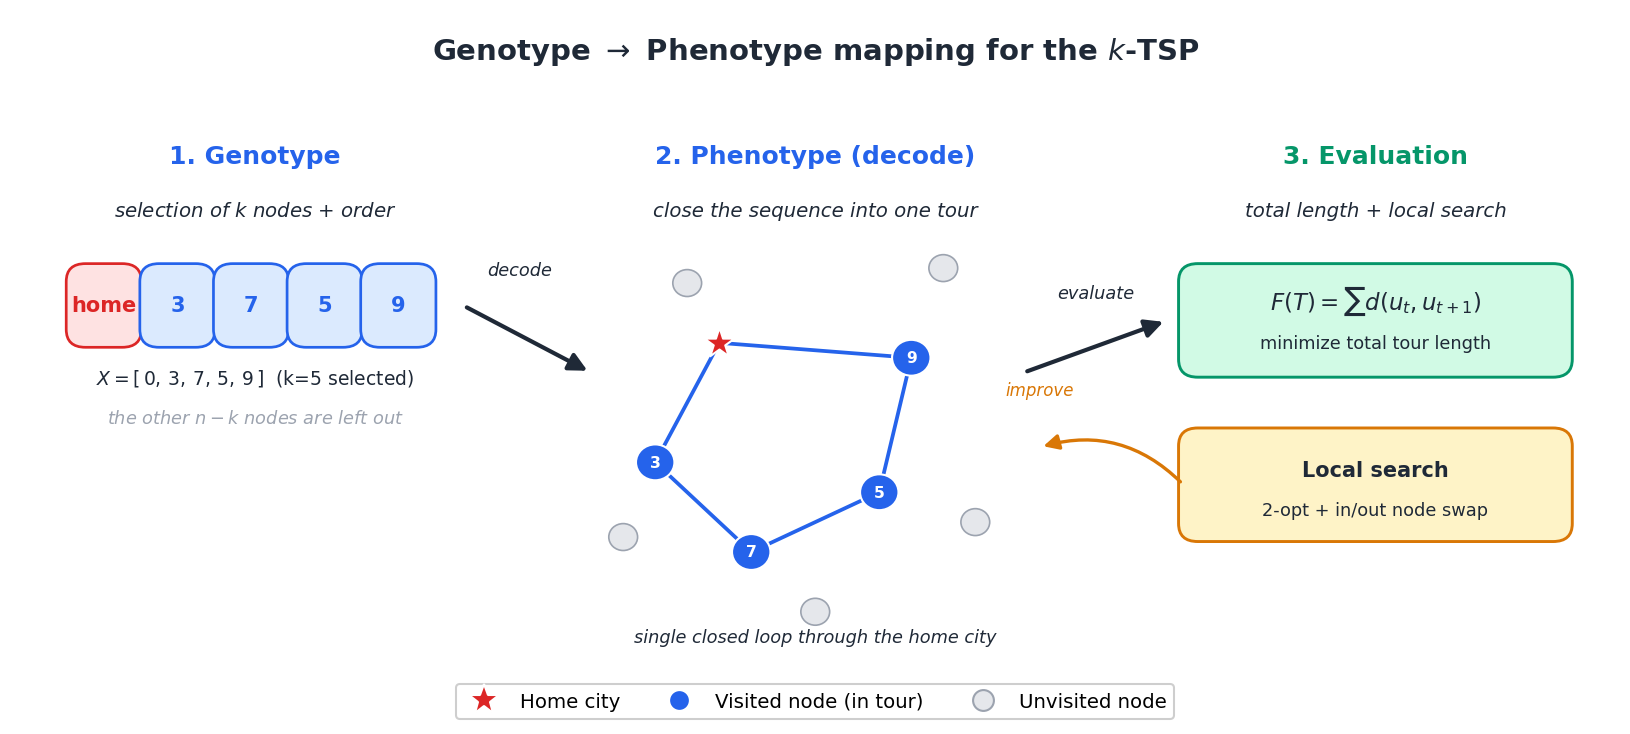
\includegraphics[width=0.85\linewidth]{figs/Genotipo-Fenotipo.png}
    \caption{Genotype$\rightarrow$phenotype flow: the genotype encodes the selected
    subset of $k$ nodes and their order; decoding closes the sequence into a single
    tour through the home city, evaluated by its total length and refined by local
    search}
    \label{fig:genphen}
\end{figure}

\paragraph{Greedy (cheapest insertion).} Starting from the home city, the tour
grows by repeatedly inserting the node with the smallest marginal insertion cost
$\Delta(v,u\!\to\!w)=d(u,v)+d(v,w)-d(u,w)$ at its best position, until it contains
$k$ nodes; it is then refined by the common local search. Several deterministic
restarts (different second nodes) keep the best tour \citep{rosenkrantz1977,gutin2002greedy}.

\paragraph{GRASP / multi-start.} Following the GRASP framework
\citep{feo1995grasp}, a randomized greedy construction picks, with controlled
noise, nodes close to the home city, builds a tour and applies local search; the
best tour over many restarts within the time budget is kept.

\paragraph{Genetic Algorithm (GA).} Each individual encodes the subset and its
order \citep{holland1975adaptation}. The GA uses binary-tournament selection, a
subset-aware crossover that repairs cardinality, a mutation that swaps positions
and exchanges in-/out-of-tour nodes, elitism and optional 2-opt refinement
\citep{potvin1996}. Because crossover and mutation change \emph{which} nodes are
selected, the GA explores the selection space as well as the ordering space.

\paragraph{Nearest Neighbor (NN).} The classic constructive heuristic
\citep{rosenkrantz1977}: from the home city the tour moves to the nearest
not-yet-visited node until $k$ nodes are selected, then is refined. Ties are broken
by node index, so NN is deterministic.

\paragraph{Nearest and Farthest Insertion (NI, FI).} Two members of the insertion
family \citep{rosenkrantz1977,bentley1992}. Both place the incoming node at its
cheapest position; they differ in which outside node is inserted next --- the one
\emph{closest} to the tour (NI) or \emph{farthest} from it (FI). Both are
deterministic.

\paragraph{Random Insertion (RI).} A stochastic multi-start insertion variant
\citep{rosenkrantz1977}: the node to insert is chosen uniformly at random and
placed at its cheapest position; the best tour over many restarts is kept.

\paragraph{Simulated Annealing (SA).} A single-solution metaheuristic
\citep{kirkpatrick1983,cerny1985}. From a Nearest-Insertion tour, SA explores the
2-opt and in/out-exchange neighbourhoods, accepting a move with cost change
$\Delta$ always if $\Delta<0$ and otherwise with probability $\exp(-\Delta/T)$,
with $T$ cooled geometrically.

\paragraph{Tabu Search (TS).} A memory-based metaheuristic
\citep{glover1986,gloverlaguna1997,knox1994}. From a Nearest-Insertion tour, at
each iteration TS applies the best non-tabu move in the same two neighbourhoods;
the attributes of applied moves are stored in a tabu list of fixed tenure, with an
aspiration criterion that overrides the tabu status when a move yields a new global
best.

\paragraph{DCIH (proposed).} The Deterministic Cheapest-Insertion Heuristic
(Algorithm~\ref{alg:dci}) builds the tour by cheapest insertion with ties broken by
node index (Phase~1) and then refines it deterministically (Phase~2). Given the same
instance it always returns the same tour, with no random seed, which makes it fully
reproducible.

\begin{algorithm}[t]
\DontPrintSemicolon
\KwIn{nodes $V$, home $0$, count $k$, distances $d$, optional candidate window $w$}
\KwOut{tour $T$ over exactly $k$ nodes minimizing total length}
\tcp{Phase 1 --- deterministic cheapest-insertion selection + ordering}
$P \leftarrow V\setminus\{0\}$\;
\If{$w>0$ \textnormal{and} $w<|P|$}{$P \leftarrow$ the $w$ nodes nearest to $0$}
$s \leftarrow \arg\min_{v\in P}\,(d(0,v),\,v)$ \tcp*{tie-break by node index}
$T \leftarrow [\,0,\,s\,]$;\quad $P\leftarrow P\setminus\{s\}$\;
\While{$|T| < k$ \textnormal{and} $P\neq\varnothing$}{
  \ForEach{$v\in P$ \textnormal{(increasing index)}}{
    \ForEach{adjacent pair $(a,b)$ in cyclic $T$}{
      $\Delta \leftarrow d(a,v)+d(v,b)-d(a,b)$; keep smallest $(\Delta,v,\text{pos})$\;
    }
  }
  insert the best $v$ at its best position; remove $v$ from $P$\;
}
\tcp{Phase 2 --- deterministic local refinement}
$T \leftarrow \textsc{TwoOptCycle}(T,d)$\;
\Repeat{no improvement}{
  $T \leftarrow \textsc{SwapInOut}(T,d)$; \ \ $T \leftarrow \textsc{TwoOptCycle}(T,d)$\;
}
\Return{$T$}\;
\caption{DCIH for the $k$-TSP}\label{alg:dci}
\end{algorithm}

As a near-optimal reference we use the Lin--Kernighan--Helsgaun solver
\citep{Helsgaun,lin1973}, whose extension LKH-3 \citep{helsgaun2017lkh3} supports
the $k$-TSP natively; the best-known solutions (BKS) are those obtained by LKH-3 on
the benchmark of \citet{pandiri2020}. LKH-3 is used only as the reference and is
not among the methods competing under the time budget.

\section{Experimental setup}\label{sec:setup}

To make our results directly comparable with the state of the art, we follow the
exact experimental protocol of \citet{pandiri2020}. The benchmark comprises the
\textbf{76 TSPLIB instances} \citep{TSPLIB} of that study, with sizes from $n=14$
to $n=783$. For each instance, three $k$ scenarios are evaluated: \emph{Small}
$k=\lfloor n/4\rfloor$, \emph{Medium} $k=\lfloor n/2\rfloor$ and \emph{Large}
$k=\lfloor 3n/4\rfloor$, giving $76\times 3 = 228$ test cases. Two wall-clock
termination criteria are used: a \textbf{short run} (SR) of $0.05\,n$ seconds and a
\textbf{long run} (LR) of $0.2\,n$ seconds. Every stochastic method is executed
\textbf{ten} independent times per case and the best tour is reported; the
deterministic constructions (NN, NI, FI, DCIH) are run once, as repeated runs would
return the identical tour.

Solution quality is measured by the relative gap to the LKH-3 best-known solution,
$\mathrm{gap}\% = 100\,(\text{length}-\text{BKS})/\text{BKS}$, where lower is
better and a gap of $0$ means the method matches LKH-3. For the statistical
comparison between algorithms we use the two-tailed \textbf{Wilcoxon signed-rank
test} \citep{knox1994} on the paired per-instance gaps, the non-parametric paired
test recommended for this setting. All methods were implemented in Python and share
the same distance routines and local-search core; the implementation and scripts
needed to regenerate every table and figure are released in the project repository.

\section{Results and discussion}\label{sec:results}

Table~\ref{tab:gap} reports the mean relative gap to LKH-3 over the 76 instances
for every method, termination criterion and $k$ scenario, alongside the published
results of \citet{pandiri2020} (marked with *). Fig.~\ref{fig:gap} visualizes the
same aggregates for the strongest methods, and Fig.~\ref{fig:box} shows the
distribution of per-instance gaps under the long run.

\begin{table*}[t]
\centering
\caption{Mean relative gap (\%) to the LKH-3 best-known solution, averaged over the 76 TSPLIB instances, for each termination criterion (SR $=0.05n$ s, LR $=0.2n$ s) and $k$ scenario. Methods marked with * are the published results of Pandiri and Singh (2020). Lower is better; the best value in each column is in bold}
\label{tab:gap}
\begin{tabular}{l rrr rrr}
\hline
 & \multicolumn{3}{c}{Short run (SR)} & \multicolumn{3}{c}{Long run (LR)} \\
\cline{2-4}\cline{5-7}
Method & Small & Medium & Large & Small & Medium & Large \\
\hline
Greedy & 4.73 & \textbf{9.11} & 11.59 & 4.46 & 8.43 & 10.41 \\
GRASP & 14.26 & 14.72 & 13.34 & 13.12 & 13.80 & 12.43 \\
GA & 18.46 & 14.42 & 11.05 & 13.82 & 10.49 & 8.70 \\
NN & 19.48 & 20.54 & 15.46 & 19.48 & 20.54 & 15.46 \\
NI & 16.82 & 19.38 & 18.78 & 16.82 & 19.38 & 18.78 \\
FI & 102.34 & 57.52 & 34.05 & 102.34 & 57.52 & 34.05 \\
RI & 42.57 & 23.26 & 13.47 & 38.48 & 21.94 & 12.25 \\
SA & 10.06 & 12.80 & 13.19 & 9.79 & 12.42 & 12.86 \\
TS & 7.04 & 10.13 & \textbf{11.00} & 6.23 & 9.08 & 9.42 \\
DCIH & 15.45 & 20.11 & 17.06 & 15.45 & 20.11 & 17.06 \\
GVNS* & 12.97 & 24.96 & 23.03 & 6.51 & 14.07 & 15.71 \\
HH\_RAND* & \textbf{3.09} & 9.56 & 11.55 & \textbf{2.42} & \textbf{4.50} & \textbf{6.22} \\
HH\_GREEDY* & 3.87 & 11.29 & 13.21 & 2.97 & 5.22 & 7.07 \\
\hline
\end{tabular}
\end{table*}


\begin{figure*}[t]
    \centering
    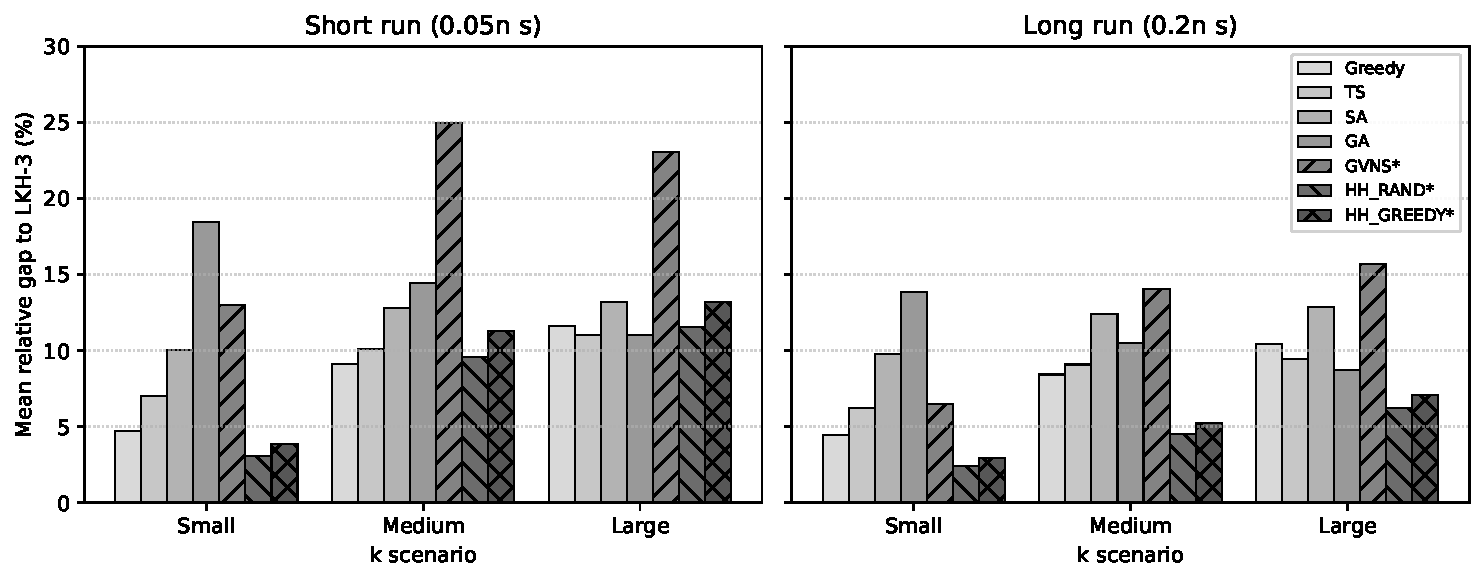
\includegraphics[width=\textwidth]{figs/Fig1_gap_scenario.pdf}
    \caption{Mean relative gap to LKH-3 (\%) by $k$ scenario, for the short run
    (left) and long run (right). Our methods (solid bars) are shown next to the
    published GVNS and hyper-heuristics of Pandiri and Singh (hatched bars, *)}
    \label{fig:gap}
\end{figure*}

\begin{figure*}[t]
    \centering
    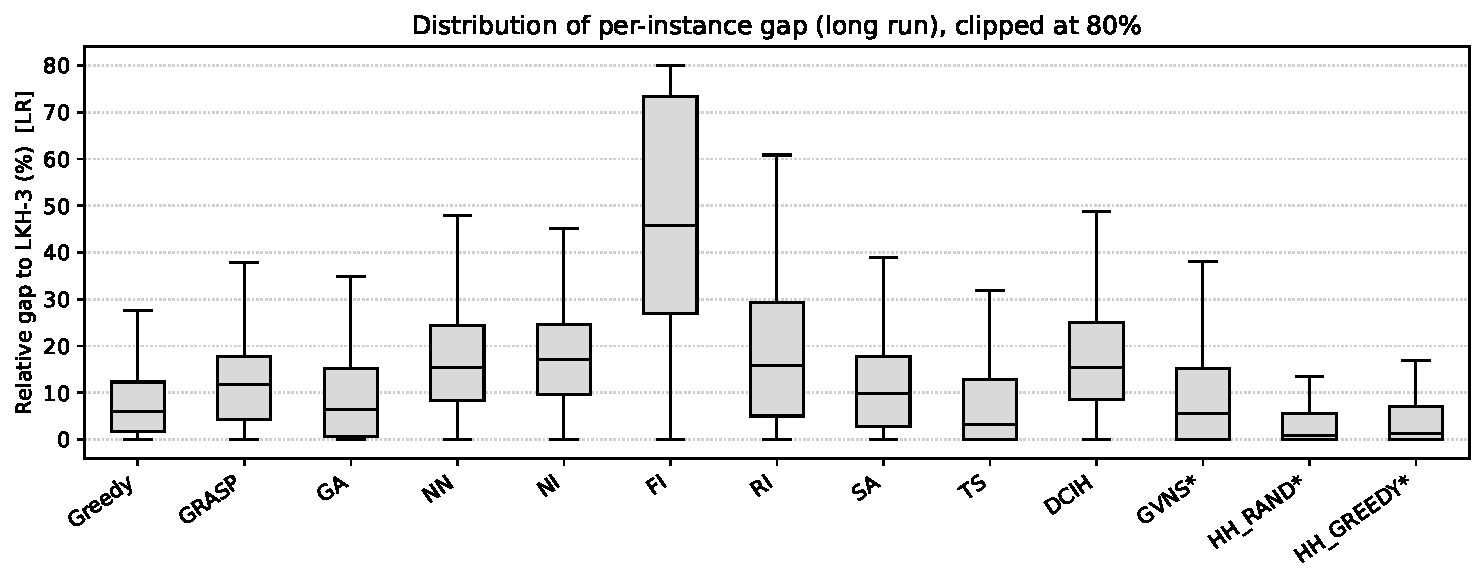
\includegraphics[width=\textwidth]{figs/Fig2_boxplot_gap.pdf}
    \caption{Distribution of the per-instance relative gap to LKH-3 under the long
    run, aggregated over the three $k$ scenarios (whiskers without outliers; values
    clipped at 80\% for readability). Methods marked * are those of Pandiri and
    Singh}
    \label{fig:box}
\end{figure*}

\paragraph{Overall ranking.} Averaged over all six groups, the hyper-heuristics of
\citet{pandiri2020} remain the strongest (HH\_RAND $6.2\%$, HH\_GREEDY $7.3\%$),
immediately followed by our \emph{Greedy} cheapest-insertion heuristic ($8.1\%$)
and \emph{Tabu Search} ($8.8\%$). Both of these clearly outperform the GVNS of the
same study ($16.2\%$). Simulated Annealing ($11.8\%$), the genetic algorithm
($12.8\%$) and GRASP ($13.6\%$) form a middle group, while DCIH ($17.5\%$) provides
a fully deterministic alternative of quality comparable to the insertion
constructions. Random Insertion and, especially, Farthest Insertion are the weakest:
inserting the farthest node is counter-productive for the $k$-TSP, where cheap-to-include
nodes should be preferred.

\paragraph{Effect of the time budget.} The deterministic constructions do not
change between SR and LR, whereas the time-driven methods improve under the long
run. The genetic algorithm benefits the most in the \emph{Large} scenario, where
its mean gap falls from $11.0\%$ (SR) to $8.7\%$ (LR), becoming the best of our
methods there. Greedy and TS are the most robust across scenarios and budgets,
staying near or below $10\%$ in most groups.

\paragraph{Comparison with the state of the art.} Table~\ref{tab:wilcoxon} reports
the Wilcoxon signed-rank test between our two strongest methods and the three
approaches of \citet{pandiri2020}. Both Greedy and TS are \emph{significantly
better than GVNS} under both termination criteria ($p<0.05$). Under the short run,
our Greedy heuristic is even significantly better than HH\_GREEDY, and TS is
statistically on par with it; the randomized hyper-heuristic HH\_RAND remains ahead.
Under the long run, with more time available, the hyper-heuristics pull clearly
ahead of our single-core methods. Counting per-case wins and ties, the best of our
ten methods matches or beats the best of the three Pandiri methods in $103$ of the
$228$ short-run cases ($45\%$) and, against HH\_GREEDY alone, in $123$ of $228$
cases ($54\%$). These results show that simple, reproducible heuristics built on a
common local-search core are competitive with dedicated metaheuristics on this
benchmark, and that they decisively outperform the GVNS baseline.

\begin{table}[t]
\centering
\caption{Two-tailed Wilcoxon signed-rank test (paired on the per-instance relative gap over the 76 instances) between our two strongest methods and the approaches of Pandiri and Singh (2020). A negative $\Delta$ means our method has a smaller (better) mean gap; $p<0.05$ denotes a significant difference}
\label{tab:wilcoxon}
\begin{tabular}{llrrc}
\hline
Crit. & Comparison & $\Delta$ gap (\%) & $p$-value & Better \\
\hline
SR & Greedy vs GVNS & -11.84 & 0.011 & Greedy \\
SR & Greedy vs HH\_RAND & +0.41 & $<$0.001 & HH\_RAND \\
SR & Greedy vs HH\_GREEDY & -0.98 & $<$0.001 & Greedy \\
SR & TS vs GVNS & -10.93 & $<$0.001 & TS \\
SR & TS vs HH\_RAND & +1.32 & $<$0.001 & HH\_RAND \\
SR & TS vs HH\_GREEDY & -0.07 & $<$0.001 & TS \\
\hline
LR & Greedy vs GVNS & -4.38 & 0.048 & Greedy \\
LR & Greedy vs HH\_RAND & +3.33 & $<$0.001 & HH\_RAND \\
LR & Greedy vs HH\_GREEDY & +2.63 & $<$0.001 & HH\_GREEDY \\
LR & TS vs GVNS & -3.96 & $<$0.001 & TS \\
LR & TS vs HH\_RAND & +3.74 & $<$0.001 & HH\_RAND \\
LR & TS vs HH\_GREEDY & +3.04 & $<$0.001 & HH\_GREEDY \\
\hline
\end{tabular}
\end{table}


\section{Conclusions}\label{sec:conclusions}

We presented a reproducible comparison of ten methods for the $k$-TSP, evaluated on
the 76-instance TSPLIB benchmark and the short-/long-run time protocol of
\citet{pandiri2020}, with LKH-3 as the best-known-solution reference and a
Wilcoxon signed-rank analysis against the published GVNS and hyper-heuristic
results. The greedy cheapest-insertion heuristic and Tabu Search are the most
robust of our methods and are significantly better than GVNS under both time
budgets; under the short run the greedy heuristic also matches or exceeds the
HH\_GREEDY hyper-heuristic. The genetic algorithm is most competitive when $k$ is
large and more time is available, while Farthest Insertion is the weakest choice
for this selective problem. The proposed DCIH offers a deterministic,
fully reproducible alternative of moderate quality. Future work includes hybrid
metaheuristics combining the greedy construction with memory-based search,
per-instance parameter tuning, dedicated node-selection rules, and an extension of
the benchmark to larger instances.


\backmatter

\bmhead{Statements and Declarations}

\noindent\textbf{Competing interests.} The authors declare that they have no
competing interests.

\noindent\textbf{Funding.} The authors received no specific funding for this work.

\noindent\textbf{Data and code availability.} The benchmark instances are the
publicly available TSPLIB instances used by Pandiri and Singh (2020). The source
code and the scripts that regenerate every table and figure are available in the
project repository.

\noindent\textbf{Author contributions.} N.\ Barrientos designed and implemented the
methods and experiments and drafted the manuscript. G.\ Gatica supervised the work
and reviewed the manuscript. Both authors read and approved the final version.

\bibliography{sn-bibliography}

\end{document}
